%NOTE: This doc formatted according to http://ec.europa.eu/research/participants/data/ref/h2020/call_ptef/pt/2018-2020/h2020-call-pt-erc-stg-2019_en.pdf

\documentclass[11pt,a4paper]{article}
\usepackage[left=2.0cm,top=2.0cm,right=2.0cm,bottom=1.5cm]{geometry}               
%\usepackage[subtle]{savetrees}
\usepackage[bibbreaks=normal, paragraphs=normal, floats=tight, mathspacing=tight, lists=tight, title=tight, margins=normal, wordspacing=normal, tracking=tight, charwidths=normal, bibnotes=normal, mathdisplays=tight, leading=tight, indent=tight, bibliography=normal, sections=tight]{savetrees} 

\usepackage{graphicx}
\usepackage{amssymb}
\usepackage{epstopdf}
\usepackage{xspace}     
\usepackage{wrapfig}
\setlength\intextsep{0pt}

\usepackage{color}
\usepackage{colortbl}
\usepackage{amsmath} % Adds a large collection of math symbols                  
\usepackage{ifthen} % for conditional statements               
\usepackage{amssymb}
\usepackage{amsfonts}
\usepackage{upgreek} % Adds in support for greek letters in roman typeset       
\usepackage{titling}
\usepackage{makecell}
\usepackage{pgfgantt}
\usepackage{lscape}
\usepackage{multirow}
\usepackage{titlesec}
\usepackage{url,amsmath,booktabs,hepunits,abhepexpt,abhep,xcolor}
\usepackage[colorlinks]{hyperref}    % Hyperlinks in references
\usepackage[all]{hypcap} % Internal hyperlinks to floats.
   

\newboolean{uprightparticles}
\setboolean{uprightparticles}{false} %Set to true to get roman particle symbols

%If we need more space we can investigate: https://tex.stackexchange.com/questions/273086/use-smaller-headheight-in-fancyhdr, https://tex.stackexchange.com/questions/271159/turn-off-fancyhdr-auto-spacing
\usepackage{fancyhdr}

\usepackage{rotating}

%\usepackage{fancyheadings}
\pagestyle{fancy}


% Playing with the page size 

\usepackage{array}
\newcolumntype{y}[1]{>{\raggedleft\arraybackslash}p{#1}}

%\renewcommand*{\arraystretch}{1.2}

%TB
%\addtolength{\oddsidemargin}{-10pt}
%\addtolength{\evensidemargin}{-10pt}
%\addtolength{\textwidth}{25pt}
%\addtolength{\textheight}{76pt}
%end TB

%\addtolength{\textfloatsep}{-2pt}
\setlength{\droptitle}{-44mm}

\setlength{\headwidth}{\textwidth}


\newboolean{articletitles}
\setboolean{articletitles}{false}

\usepackage{cite}
\usepackage{mciteplus}

\newboolean{inbibliography}

\titlespacing{\section}{0pt}{4pt}{0pt}
\titlespacing{\subsection}{0pt}{4pt}{0pt}
\titlespacing{\subsubsection}{0pt}{4pt}{0pt}

%\titlespacing{\section}{0pt}{\parskip}{0pt}
%\titlespacing{\subsection}{0pt}{\parskip}{0pt}
%\titlespacing{\subsubsection}{0pt}{\parskip}{0pt}


\title{{\Large Case for ERC Consolidator grant}}
\author{{\normalsize Caterina Doglioni}}
\date{}                                           % Activate to display a given date or no date

\usepackage[parfill]{parskip}

\begin{document}
\lhead{{\small Doglioni}}
\chead{{\small Part B1}}
\rhead{{\small REALDARK}}
\begin{center} 

{\Large\bf ERC Consolidator Grant 2020} \\
	{\Large\bf Research Proposal [Part B1]}  \\
 
\vspace{2cm} 
{\huge {\bf }}   \smallskip  

\vspace{2cm} 
{\Huge{REALDARK}} \\ 
\vspace{1cm} 
\vspace{1cm}
\end{center} 
\begin{tabular}{rcl}
Principal Investigator & : & Dr.~Caterina~Doglioni \\
Host Institution & : & Lund University \\ 
Proposal duration in months & : & 60 \\
\end{tabular}  
\vspace{2cm}


\begin{center} {\bf Summary}  \end{center}
%Up to 2000 chars...

The nature of 85\% of the matter in the universe is unknown. I will enable the ATLAS experiment to record data for a broad program of searches for this \textit{dark matter}, expanding upon the innovative techniques that I have pioneered in my ERC Starting Grant DARKJETS. 
The searches I will perform using this unique dataset will provide complementary and valuable input to the dark matter community worldwide, in terms of both technological advancements in data taking and high-impact physics outputs. 

[Add more here...]

\clearpage

\section*{Section A: Extended synopsis of the proposal} 

\medskip

\section{Aims and impact of this research project} 
\smallskip

The first years of data taking at the Large Hadron Collider (LHC)~\cite{LHC2008} at CERN yielded the discovery of a new fundamental particle, the Higgs boson~\cite{Khachatryan:2016vau}. With this and other notable results, the LHC data has confirmed the predictive power of the Standard Model (SM) of particle physics, the theory of fundamental particles and non-gravitational interactions. However, the amount of ordinary matter described by the SM is exceeded by a factor of five by a kind of unknown matter as determined by cosmological observations, called Dark Matter (DM)~\cite{Bertone:2016nfn}. 

%My big idea is to expand on successful searches for DM that I pioneered to look elsewhere because now it's the time to expand that program. 

Theoretical models that explain the abundance of DM in the universe include massive DM particles that interact weakly with ordinary particles, called WIMPs. These can be produced at the LHC in collisions of ordinary matter (see e.g.~\cite{Boveia:2018yeb} and references therein). 
Creating DM in controlled conditions enables the study of its interactions with ordinary matter, complementing searches for cosmological DM in direct and indirect detection experiments and astrophysical observations. %~\cite{Boveia:2018yeb}. 
WIMP Dark matter searches have been a flagship of the physics programmes of LHC experiments. In my Starting Grant I have led novel and comprehensive searches for particles that could reveal SM-DM interactions. I have ensured that the world-leading LHC constraints that resulted had a widespread impact in the global quest for DM, within a consistent theoretical framework that has been adopted by most LHC WIMP searches so far~\cite{DMWG}.  

Lack of evidence for WIMPs so far motivates a two-prong approach for DM searches at the LHC. In this Consolidator Grant proposal:
\begin{itemize}
    \item I will advance the state of the art for WIMP searches by enhancing their sensitivity to probe the rarest SM-DM interactions.
    \item I will deliver a new set of searches for models beyond the WIMP paradigm. These models postulate a new force akin to the strong interaction in the SM and could have so far escaped detection. 
\end{itemize}

The discovery of new, rare processes, at a time when traditional data-taking methods confirm the SM, mandates technical innovation. The LHC collides bunches of protons up to 30 million times per second. Recording and processing all this data is unfeasible: only a small fraction of interesting data can be selected by the experiment’s \textit{trigger systems} due to budgetary constraints on both processing and storage; the rest is discarded forever. This leads to a loss of sensitivity to large areas of parameter space for DM models. 

%USED BELOW These budgetary constraints make it difficult to extend the physics programme using standard techniques, requiring a paradigm shift in the way in which data selected and processed.
%Current data taking methods do not provide sensitivity to large areas of parameter space for DM models. 
The searches in this proposal will be enabled by innovative data-taking techniques at the earliest stage of data selection and processing, that increase the utility of the data recorded by the ATLAS experiment as a whole. These techniques, called Trigger Level Analysis (proof-of-principle delivered by my StG~\cite{PRL}) and Partial Event Building in ATLAS, reduce the size of the data used for physics analysis by a factor of \color{red}X\color{black}, overcoming the storage limitations that would otherwise force ATLAS and other LHC experiments to discard the majority of data of interest for many DM searches. %milliseconds after being taken
%taken, and deliver a dataset with unprecedented sensitivity. 

The physics results from this project, derived analysis products, and tools for their interpretation will be disseminated to the broader DM community in order to generate interdisciplinary impact.
%~\cite{Bertone:2018xtm}. 
%\end{itemize}
%	\item by exploiting the unprecedented sensitivity of the data recorded with these techniques by leading a comprehensive set of searches for DM models beyond the WIMP paradigm that . I will lead searches for new DM candidates and associated particles, which until now have escaped detection; % in this first phase of LHC data taking
%	\item by disseminating
The outcomes of this proposal will have a transformative effect in terms of both data taking innovations and in the global quest for DM. 
Data storage requirements are a widespread concern for LHC upgrades, as well as for many experiments where the increase in data collection is not matched by a proportional increase in resources~\cite{HSF}. 
This proposal will directly address this challenge, and develops solutions that can be ported beyond the LHC. 
Future collider projects will be prioritized in this decade~\cite{EuropeanStrategy}, and a number of astroparticle and non-collider experiments will start taking data~\cite{Astro2020}. 
This proposal delivers as outputs discoveries or constraints that are usable for these scientific communities by using Open Science tools, defining the future direction of DM research. 
% within the DM research community,
% Mention that HSF says RTA is crucial for 2020
% Mention that DM people says that they want this stuff done

%and thanks to the presence of a strong theory group with world-leading expertise in the DM models I intend to look for. 
\section{Organization of the project} 

\smallskip


%CAN BE USED This proposal will solve this issue by enabling the ATLAS experiment to record data in a new manner. This will permit, for the first time, this wealth of recorded data to be used for early measurements and new dark matter searches, and propagates the results and the developed tools to the broader community. \textbf{Mention the tools somewhere}

%\begin{wrapfigure}{L}{0.35\textwidth} 
\begin{figure}[h!]
\begin{center}
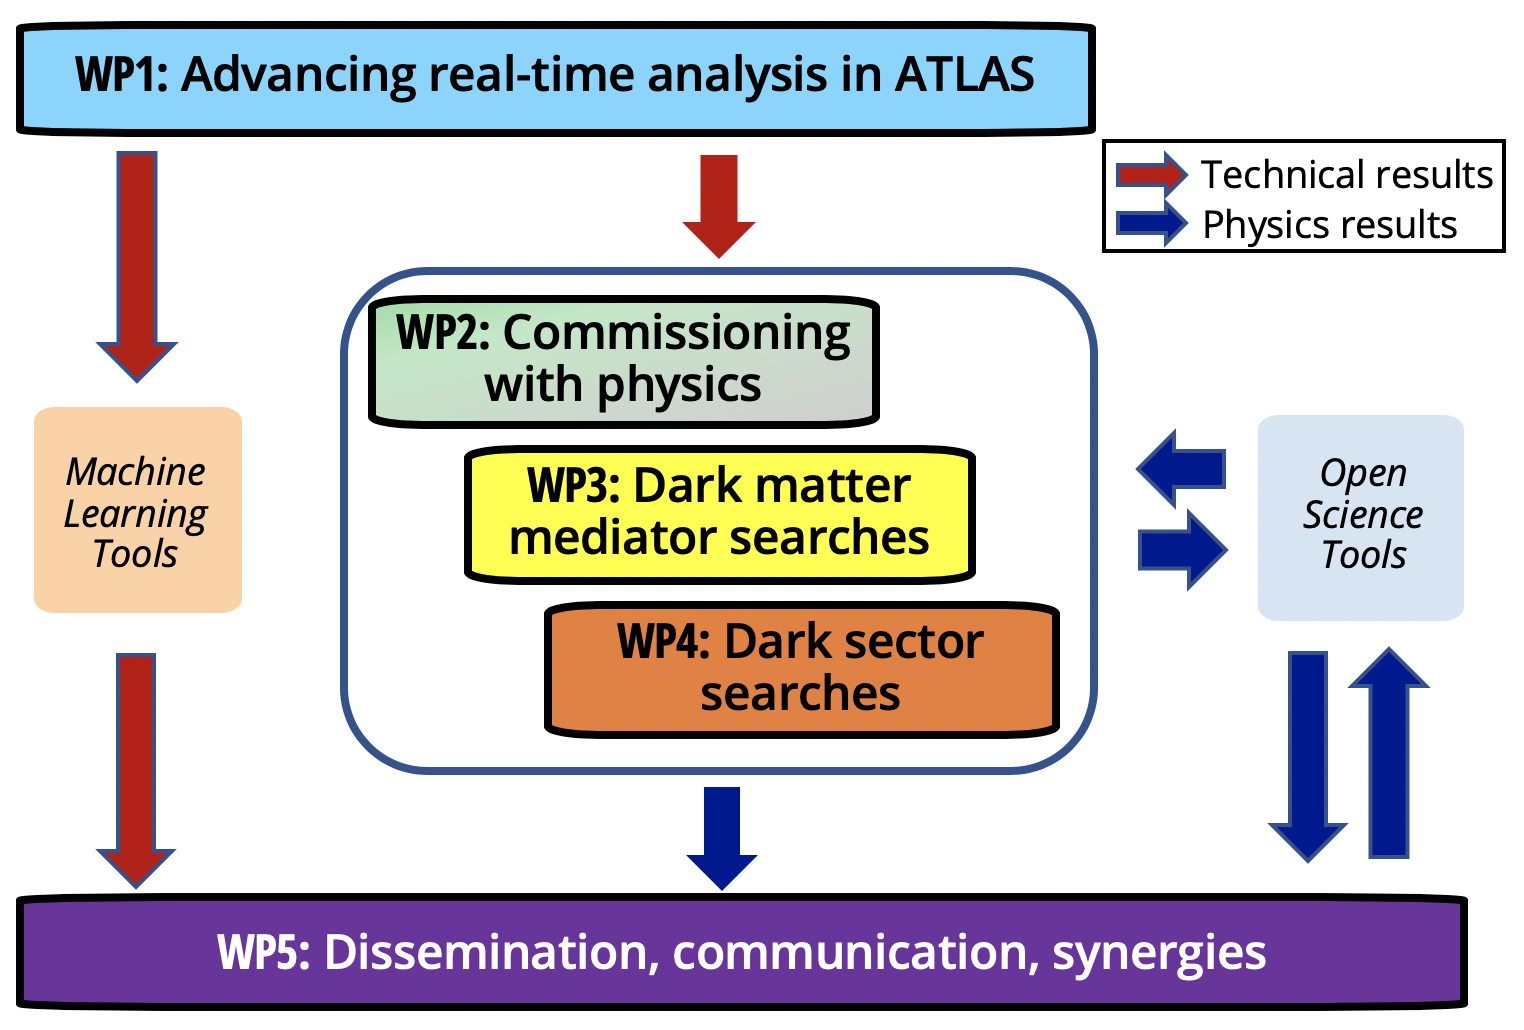
\includegraphics[width=0.5\textwidth]{figs/WPs_shorter}
\caption{\label{fig:WPs} \footnotesize Schema of work packages and expected results.\color{red} This will become an in-line figure, possibly on the 1st page, after feedback. If needs be, the first section will be shortened. \color{black}}
\end{center}
%\end{wrapfigure}
\end{figure}

The proposal consists of five logically interconnected work packages.
%to maximise impact. 
The work packages and their interconnections are indicated in Fig.~\ref{fig:WPs}. In \textbf{WP1} I will overcome the technological constraints that limit the sensitivity to a variety of physics phenomena including DM, with the use of non-standard data taking and recording techniques, and employ machine learning techniques for forward-looking improvements. In \textbf{WP2}, I will lead a programme of searches and measurements using the first LHC Run 3 data and in so doing commission the techniques developed in WP1. In \textbf{WP3} and \textbf{WP4}, I will use the dataset recorded with the fully commissioned techniques developed in \textbf{WP1} and \textbf{WP2} to perform world-best and world-first searches for current and state-of-the-art dark matter models. In~\textbf{WP5}, I will interpret the results of those searches in coherent frameworks that transgress model boundaries with the inclusion of input from LHC measurements and non-collider DM searches using Open Science tools, and work in synergy with the broader community for optimal dissemination of results and tools. 
%\medskip

%\clearpage
\section{Project description}
\smallskip

\subsection*{WP1: Real-time analysis in ATLAS}

%Used above? 
%The discovery of new, rare processes, at a time when traditional data-taking methods confirm the SM, requires technical innovation. The LHC collides bunches of protons up to 30 million times per second, with each bunch resulting in X proton-proton collisions. Recording and processing all this data is unfeasible: only a small fraction of interesting data can be selected by the experiment’s \textit{trigger systems}, and it must be selected in the order of milliseconds after each collision has taken place due to budgetary constraints on both processing and storage; the rest is discarded forever.

%USED ABOVE These budgetary constraints make it difficult to extend the physics programme using standard techniques, requiring a paradigm shift in the way in which data selected and processed.
%A decision on whether a collision event is “interesting” is made by the experiment's \textit{trigger system} in the order of milliseconds after the collision has taken place, and the majority of the events that are not considered interesting are discarded

%, and it must be selected in the order of milliseconds after each collision has taken place 

Two notable examples of discoveries that would be impossible due to these constraints \textbf{[not anymore because my StG, and also we shouldn’t ignore LLP searches]} in ATLAS are:
\begin{itemize} 
\item Rare processes where a new particle decays into ordinary matter, mimicked by more frequent SM-only processes that lead to the same low-level trigger signatures in the detector. These new processes are discarded together with the vast amount of irreducible SM background mimicking them;
\item Processes where new particles have non-standard interactions with ordinary matter. In these cases, the exact content of the collision is difficult and time-consuming to reconstruct within the timing budget with which a decision must be made, therefore the features that distinguish signal from background to classify the event as interesting are missing and the event is discarded.
\end{itemize}
In this proposal I will map these discoveries to two classes of models which explain the particle nature of dark matter discussed in WP3 and WP4. The data collected using these techniques represents an entirely new dataset that can extend the experimental reach of the ATLAS experiment with a similar amount of resources~\cite{Resonances}. 

The main technological advancement delivered by this proposal is to break the traditional paradigm of first recording the entirety of raw detector data and then analyzing it, to one in which data is reduced and processed in real-time, using the two following techniques:

\begin{wrapfigure}{R}{0.5\textwidth} 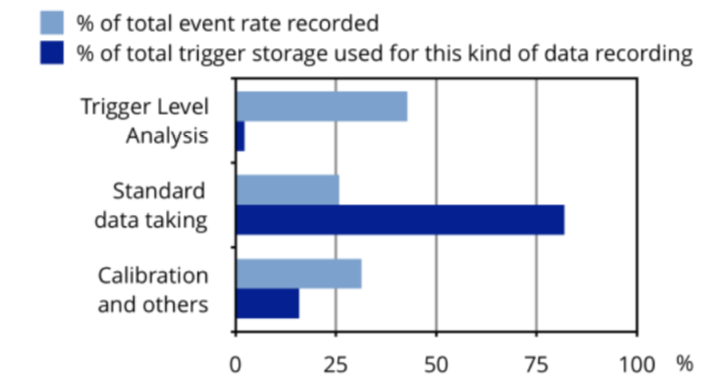
\includegraphics[width=0.5\textwidth]{figs/TLAPEB}
\caption{\label{fig:TLAPEB} \small Fraction of event rates recorded and trigger storage used for standard and Trigger Level Analysis technique. 
The event rate recorded with Trigger Level Analysis is much higher than the rate of events for standard data taking, for a much smaller amount of storage resources, as measured in 2017 ATLAS data-taking, adapted from~\cite{Computing}. \scriptsize \color{red} If available, include estimates for this proposal. If not, change colors and only include Standard data taking and Trigger Level Analysis. Also, show how much this could be compressed if compression worked (although that's an offline thing?). \color{black}}
\end{wrapfigure}


\textbf{Trigger Level Analysis}\footnote{Turbo LHCb and data scouting in CMS}. Traditional data taking methods store raw detector data in its entirety, so that it can be later reconstructed to extract higher level information. In the real-time analysis paradigm, reconstruction is performed at the first processing stages prior to making a decision, retaining only the higher-level information. As this information is considerably smaller than the raw data, this technique enables us to record a much larger number of events in the same data rate, as shown in Fig.~\ref{fig:TLAPEB}.  
With my StG, I have shown that this is effective in a proof-of-concept use case of dark matter mediators decaying into sprays of collimated particles (jets)~\cite{PRL_TLA}. Within this CoG I intend to extend this paradigm to photons, electrons and muons so that it can be used to extend the ATLAS experiment reach to a much larger set of searches and measurements. 

\textbf{Selective event reconstruction} (called Partial Event Building in ATLAS). In this technique, the information available to real-time analyses is augmented by a subset of the raw detector information in analyst-specified regions of the detector. This paradigm combines the data rate enhancements of real-time analysis with the added precision of full offline reconstruction in a user-configurable manner. Non-ordinary features signaling the presence of new phenomena can then be detected \textit{a posteriori}. This proposal will commission and use this technique for physics searches for the first time in ATLAS. 

As a pioneer of real-time analysis, I have delivered proof-of-concept studies for these techniques, but they must be now developed and commissioned on a much larger scale in order for me to exploit them for groundbreaking DM searches with the Run-3 dataset. 


Both of these techniques reduce data storage requirements, but these can be complemented by further gains in data compression. I will therefore pursue a method for data compression using machine learning algorithms where my students have made preliminary studies, in collaboration with other ATLAS ML and computing experts. This is a forward-looking activity targeting the high-luminosity LHC run starting in 2026 as well as experiments beyond the LHC (e.g. gravitational wave experiments).

%which will be undertaken by supervising Master’s students from the engineering faculty. 
\subsubsection*{WP2: Early searches and measurements}

During the shutdown between the Run-2 and Run-3 data taking periods, the ATLAS experiment trigger system is undergoing significant upgrades~\cite{FEXes}, and the software for the real-time event selection is being rewritten~\cite{MT}. 
Thorough commissioning and testing, first with simulation and cosmic ray data, and subsequently with LHC commissioning data is mandatory. The initial LHC accelerator plan for Run-3  foresees that the first two years (2021-2022) will be used as a ramp-up for the production data taking period, with the majority of the dataset being collected in (2023-2024)~\cite{SomeRandomEuropeanStrategyPresentationOrTooMuch?}. 
The first two years are the ideal opportunity to use the already-established Trigger Level Analysis from Run-2~\cite{TLAPRL} to test a completely new software framework and the performance of the detector, and document this work with physics and technical results. 

In WP2 I will select events where at least two jets are detected and reconstructed in real-time within the trigger system, and compare the performance of their reconstruction and calibration at the trigger level with traditional data taking. The reduced duty cycle of the accelerator will enable this study to record data at high rates, reducing the time-to-insight. \textbf{}.
I will make extensive use of the Open Science tool RECAST~\cite{RECAST} and Docker containers~\cite{Docker} to preserve the end-to-end analysis workflow, from detector data to final plots.  

Beyond the technical publications documenting the new software framework and its commissioning with LHC data, this WP will lead to physics publications that already break new ground with early data. 

\subsubsection*{WP3: Dark Matter mediator searches}

One of the most striking gaps in the knowledge of our universe is the nature of dark matter. All we know about dark matter so far comes from its gravitational and astrophysics observations and simulations; astrophysics also provides some tantalizing hints towards the existence of a new particle~\cite{HooperLeane} that are imperative to pursue~\footnote{Caveat about gravitation}. 

In the past decade, the most popular theoretical explanation for the particle nature of dark matter is that DM is a WIMP. This is both because the relic density of DM can be comprised by WIMPs in its entirety, and because particles behaving like WIMPs are postulated by many theories (e.g. supersymmetry)\cite{AR}. 

The first data taking period of the LHC and first generation of direct detection experiments have constrained the DM WIMP parameter space, but the search for these particles is far from over: their interactions with ordinary matter may not yet be accessible with current experiments. Therefore, collider, direct and indirect detection experiments will continue their flagship WIMP searches into the next decade and beyond, with significant upgrades and new experiments planned~\cite{Astro2020, EuropeanStrategy}. 

This WP furthers searches for WIMP models at the LHC using the Trigger Level Analysis technique, in a scenario that is not fully constrained by existing searches, by searching for the visible decays of the particles mediating the interaction between ordinary and dark matter. 

\begin{wrapfigure}{L}{0.25\textwidth} 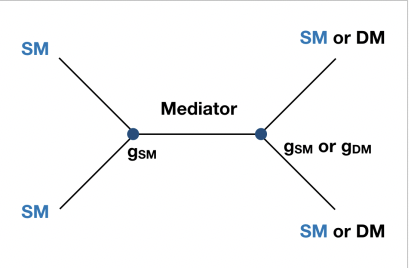
\includegraphics[width=0.25\textwidth]{figs/WIMPMediator}
\caption{\label{fig:WIMPMediator} \small Sketch of WIMP mediator model \scriptsize \color{red} Improve quality, consider adding DD/ID etc. \color{black}}
\end{wrapfigure}

WIMP DM can be produced via interactions of SM particles at the LHC through a new force mediator (analogous to the W and Z for the Weak Force), as in Fig.~\ref{fig:WIMPMediator}. Here, quarks within the colliding protons couple to a mediator particle which decays to a pair of WIMPs or, through the same interaction responsible for mediator production, to two jets. 
This model is used by the majority of DM LHC searches and can reproduce the observed relic density. It can be used as a building block for more complex theories (e.g. those mentioned in WP4) since it can describe the behavior of these processes even with a small number of parameters. 

In WP3, I will search for the decays of mediators of DM in two-jet final states, accompanied by a photon or a jet. I have pioneered LHC searches for this signature in my StG using traditional data taking techniques as a way to look for new particles with lower masses with respect to what was possible in two-jet searches with the Trigger Level Analysis, and in this CoG I will implement the TLA technique in this kind of search, relying on the first ATLAS availability of TLA photons (\textbf{WP1}). This will lead to a major improvement to the sensitivity of particles in a region of phase space where the SM massive force mediators reside ($<$ 400 GeV), that is inaccessible with the same sensitivity by other kinds of searches, and that is motivated by a number of theoretical models beyond WIMP DM~\cite{ALP, HooperLeane}.  

\subsubsection*{WP4: Mapping dark/hidden sectors}

Partly motivated by the constraints set on such particles by first-generation direct searches, and by the analyses I have led in the first phase of the LHC data taking, the DM community has recently started to generalize the flagship searches for these weakly interacting massive particles (WIMPs) by expanding the search program for particles with much weaker interactions with SM particles than what predicted by WIMP theories~\cite{FIMPs}. 
This is a strong motivation for this project to enable detection of different DM candidates with broad theoretical connections, such as new particles from dark/hidden sectors~\cite{HiddenSector}. 

While the searches in WP2 are powerful probes of WIMPs, they are not optimally sensitive to DM mediators whose interaction with the SM is even feebler. This is the case for “dark sector” or “hidden valley” models\cite{Zurek}, where the only connection between the SM and the DM particle spectrum occurs via a feebly coupled mediator particle (e.g. a photon-like particle with non-zero mass). Hidden valley models also postulate a multitude of dark sector particles, mirroring the complexity of the SM in a theory similar to the strong force.  
These "dark Quantum Chromodynamics” (dark QCD) theories, where the fundamental constituents (e.g. dark quarks) fragment into a mixture of visible and invisible particles (dark hadrons), would still give rise to jets of particles. However, the particles forming the jet may be invisible, or only emerge after having partially traversed the detector material. Dark sector jets may also contain very light dark matter mediators that decay into low-energy electrons and muons. 
Given the complexity of the parameter space driving the phenomenology of dark QCD, there are a wide range of possibility of how dark jets appear in the detector that need to be mapped. The majority of those possibilities currently escapes detection and are discarded at the trigger level, either because of the very large SM QCD  backgrounds (a problem shared by the search targets in WP3) or because the trigger system is unable to recognize their characteristic features in time and considers them noise.  
The combination of TLA and partial event reconstruction is the solution to this problem: by recording a limited set of information reconstructed at the trigger level in addition to the full set of raw data behind the dark jet, we bypass storage limitations and we can reconstruct the features that distinguish signal from background at a later stage where more resources are available. 

While the dataset collected with those techniques allows mapping a large number of dark sector models, two classes that have not been searched at the LHC before are chosen to be investigated with Run-3 data in this proposal.

In the first class, one of the dark sector particles within the dark jet can easily make up the relic density of dark matter and is therefore completely invisible to the detector, leading to a \textit{semi-visible} jet. Since the main background for this signal is composed of mismeasured QCD jets, it is crucial that both QCD jets and dark jets are calibrated so that the measurement error and jitter can be minimized. As an expert in hadronic jets and their calibration, I will develop and employ techniques tailored for this specific search. 
In the second class of models, low-energy leptons from the decays of e.g. a light dark mediator or from a dark Higgs boson are an integral part of the dark jet, mirroring the way as QCD particle showers develop an interleaved electromagnetic component. The main challenge of searches for these models is the development of reconstruction algorithms and calibrations for these leptons, and we will rely on existing algorithm that the ATLAS collaboration has already developed but not yet widely used for physics measurements and implement them in the trigger level reconstruction within WP1. 

As part of WP5, the parameter space that will be investigated in these models will be carefully chosen by considering the constraints from past searches for the individual particles within the dark jet (e.g.~\cite{DarkPion})  and LHC measurements of the development of QCD jets that are sensitive to changes in the structure of jets, using a software program that enables the use of precision results released by the ATLAS, CMS and LHCb collaboration to be used to constrain the parameter space of new physics models~\cite{CONTUR}. 

\subsubsection*{WP5: Conceptualization, contextualization, synergies}

%\begin{wrapfigure}{R}{0.5\textwidth} 
%\begin{figure}[h!]
%\begin{center}
%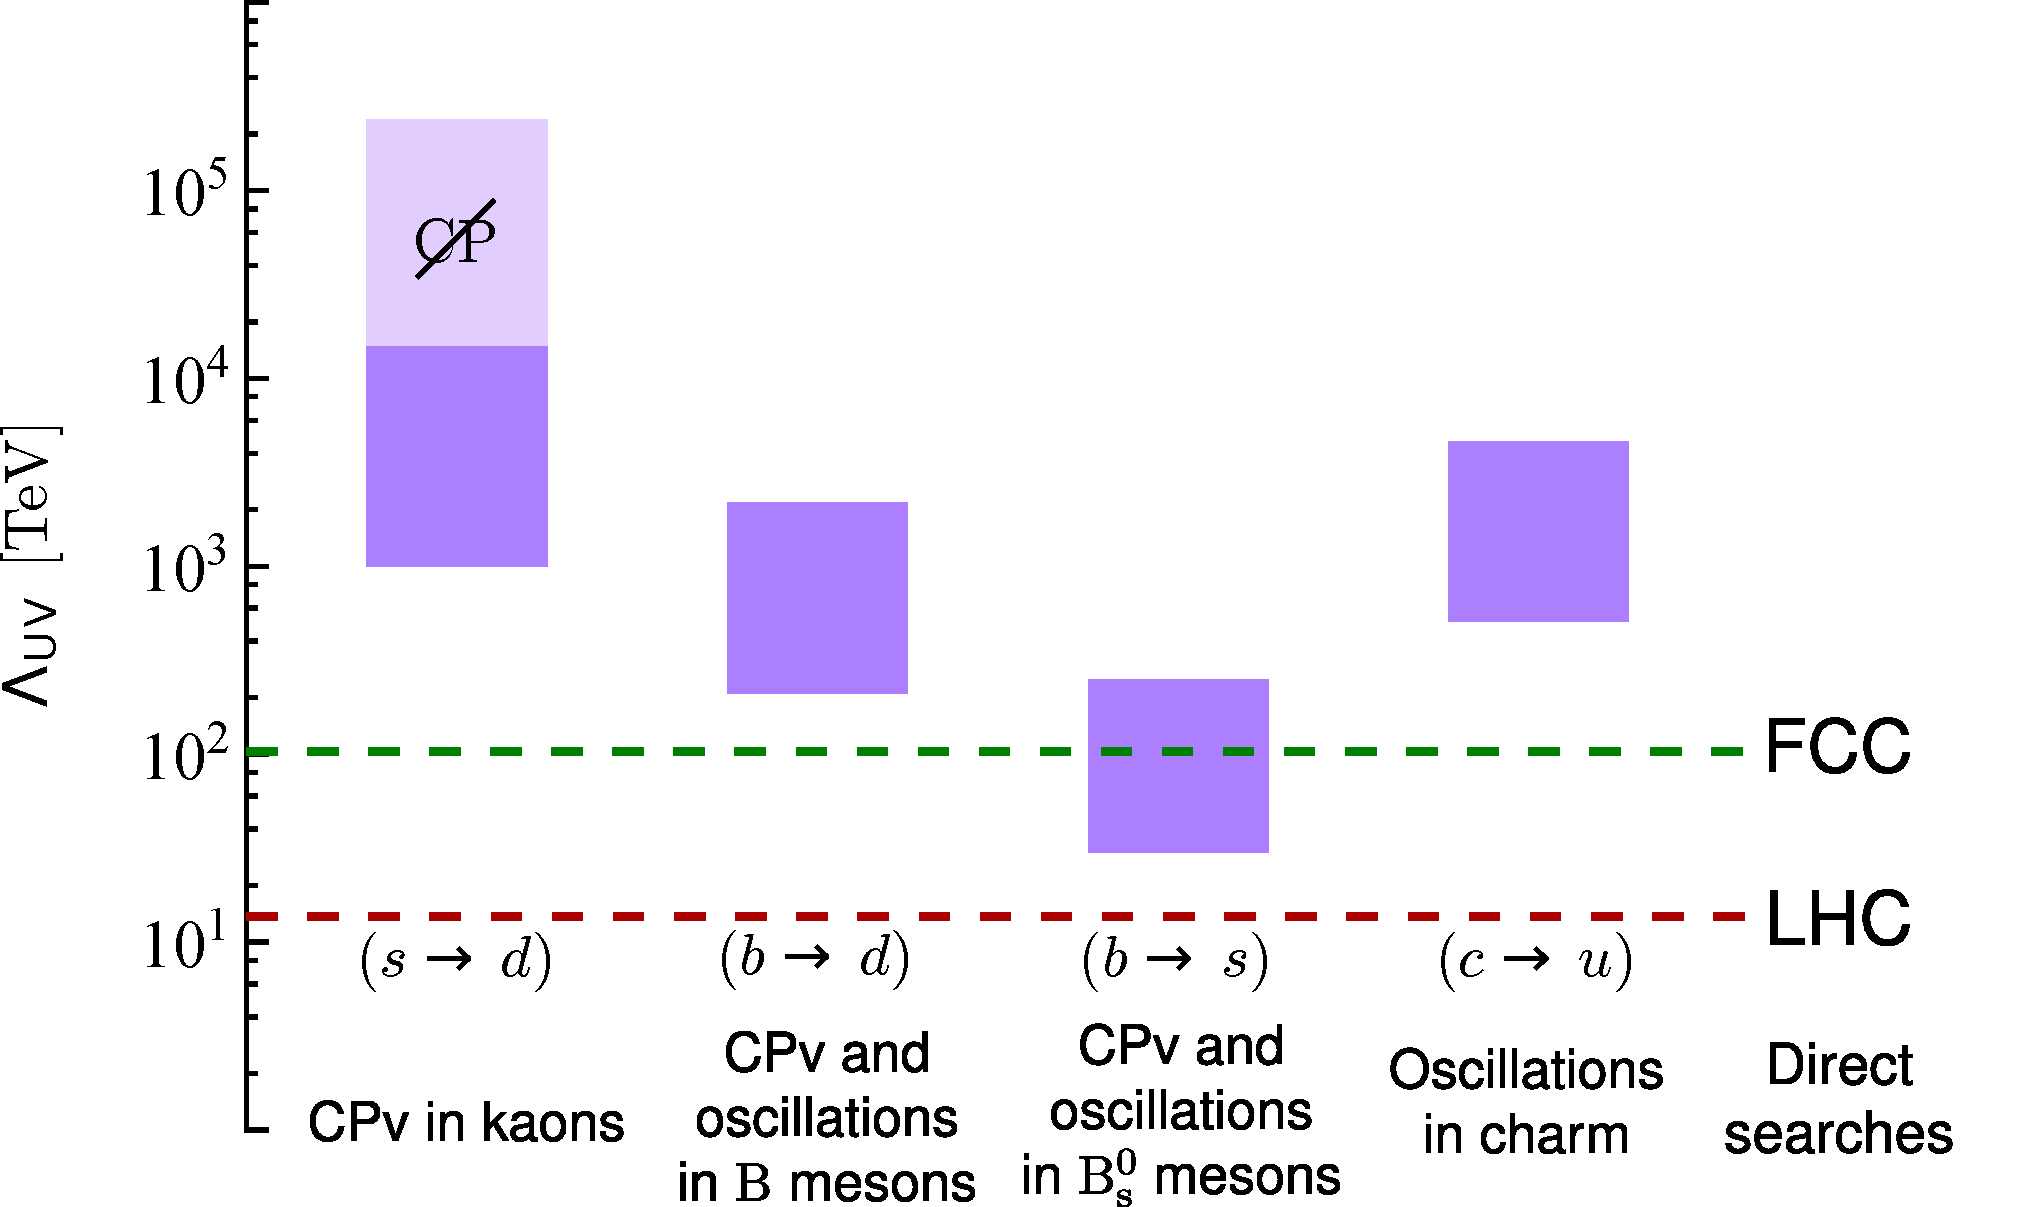
\includegraphics[width=0.7\textwidth]{figs/flavorprobes.pdf}
%\caption{\label{fig:scales} Energy scales of generic NP models probed by heavy flavor observables. The energies accessible to searches at the LHC and a potential $100~\TeV$ future collider (FCC) are indicated. Figure adapted from~\cite{neubert:scales}}
%\end{center}
%\end{wrapfigure}
%\end{figure}


\section{Timeliness of the research program and appropriateness of the PI and team} 
\smallskip

This research program spans the entire upcoming LHC data taking period (Run-3). The 2021-2026 period is the ideal time to advance the state-of-the-art in processing of large datasets and DM searches, ensuring continued impact through a significant extension of my current successful StG research program that relies on novel data-taking techniques. The LHC schedule includes an initial commissioning period where innovations can be deployed and tested via early measurements with start-up data, which forms the first part of this proposal. The second phase of this proposal will use the wealth of data delivered by the LHC during the fully-commissioned data taking period for novel DM searches, with a dataset that will be more than twice as sensitive to the physics observables of this proposal than the data collected so far. 

I am uniquely suited to deliver an ambitious and timely research program in which I will lead a research team of two postdoctoral researchers and two students, complemented by talented Lund University undergraduates that I have a track record of recruiting and training.
As evidenced by my CV and track record, my profile combines both technical and scientific proficiency with leadership of large groups of scientists in both physics and data analysis tools. 
With my international collaborators and within my StG, I have led a paradigm shift in data taking techniques in ATLAS from software concept to publication \textbf{[and I am now HSF convenor]}. I have authored a number of LHC searches for DM and new phenomena, and I have coordinated ATLAS- and LHC-wide working groups instrumental to the design of DM search strategies~\cite{DMWG}. 
As an internationally recognised expert in the field, I have been invited to write review articles on the subject area of this proposal~\cite{Buchmueller:2017qhf, Boveia:2018yeb}, and have contributed to the European Strategy update, which defines the next 10 years of Europe-wide and international research in HEP, as one of the scientific secretaries of both the Dark Matter and Beyond the Standard Model Physics Planning Groups~\cite{Strategy:2019vxc}.


% Mention who asked you to do this rather than saying who you're doing this with
%In addition to further enhancing my standing as an expert in DM, 

As a recognized expert in DM searches and collider data taking techniques with a track record of synergistic interdisciplinary activities, the impact of this proposal will not be limited to high energy physics but will be disseminated further afield to generate impact in DM direct detection and cosmological disciplines.  


\section{Project planning}
\smallskip

I will lead a research team consisting of two postdoctoral researchers and two PhD students. 

%\begin{figure}[h!]
%\begin{center}
%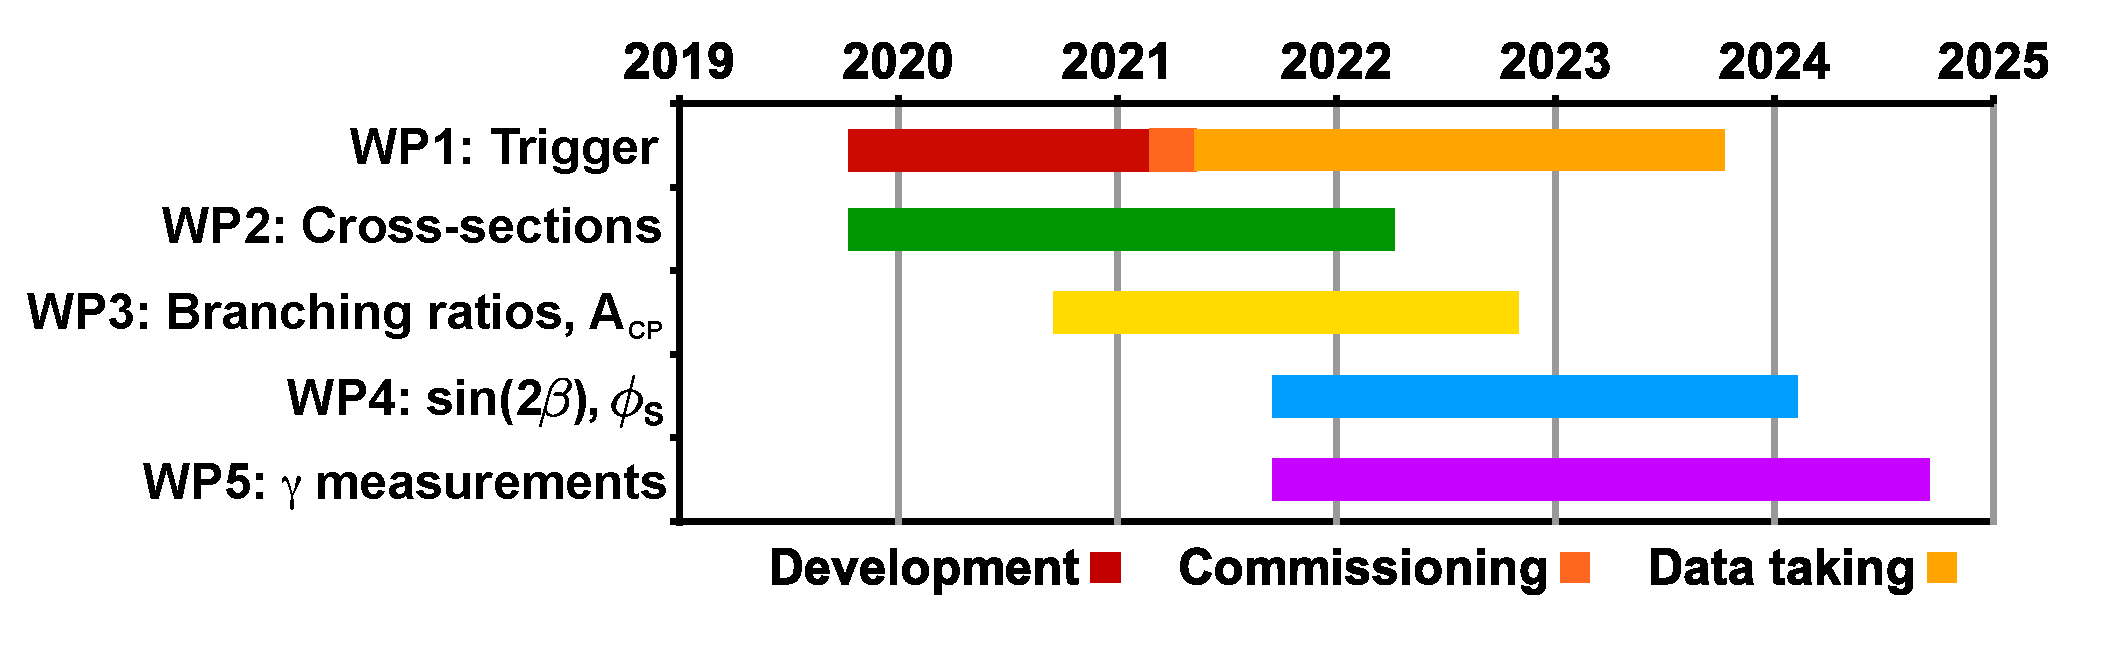
\includegraphics[width=0.7\textwidth]{figs/timeline_new.pdf}
%\caption{\label{fig:timeline} Timeline of the proposal.}
%\end{center}
%\end{figure}

%The LHC will begin Run III with a commissioning period during %which the software trigger will be exercised. A detector %commissioning paper will be published in Q2 2021, and a %performance paper in Q4 2021 where the new exclusive trigger %selections will be used to highlight the increased efficiency %with respect to Run II. 



\clearpage
%\addcontentsline{toc}{section}{References}
\setboolean{inbibliography}{true}
\bibliographystyle{LHCb}
\bibliography{researchrefs}

~ 

%{\bf Note:} The PI is acknowledged in Ref.~\cite{Jung:2014jfa} and is an author of Refs.~\cite{LHCb-PUB-2014-027,Williams:1670992} as well as of all publications by the LHCb collaboration -- Refs.~\cite{Alves:2008zz,CERN-LHCC-2014-016,LHCb:2011aa,Aaij:2013mga,Aaij:2014ywt}.
%The PI is the contact author within LHCb for Ref.~\cite{Aaij:2014ywt}.

\clearpage

%
\section*{Section B: Curriculum Vitae} 
\subsection*{Personal information}
\begin{tabular}{rlrl}
{\bf Name} & Dr.~Conor Fitzpatrick & {\bf Date of birth} & 03/10/1982 \\
{\bf Nationality} & Irish \\
{\bf ORCiD} & \hyperlink{https://orcid.org/0000-0003-3674-0812}{0000-0003-3674-0812} & {\bf inSPIRE} & \hyperlink{https://inspirehep.net/author/profile/C.Fitzpatrick.1}{C.Fitzpatrick.1}

\end{tabular}
\subsection*{Education}
\begin{flushleft}
\begin{tabular}{rl}
\bf{2012} & PhD, Experimental Particle Physics \\ 
& School of Physics and Astronomy, University of Edinburgh, UK. \\ 
& Supervisor Prof. F. Muheim \\ \\
\bf{2008} & Master of Physics with honours \\ 
& School of Physics and Astronomy, University of Edinburgh, UK. \\ 
\end{tabular}
\end{flushleft}
\subsection*{Current position}
\begin{flushleft}
\begin{tabular}{rl}
\bf{2014 - \phantom{2014}} &  Collaborateur Scientifique, Laboratoire de physique des hautes \'energies\\ 
& \'Ecole polytechnique f\'ed\'erale de Lausanne, Lausanne, Switzerland
\end{tabular}
\end{flushleft}

\subsection*{Fellowships and awards}
\begin{flushleft}
\begin{tabular}{rp{13.5cm}}
\bf{2012 - 2014} & Research Fellowship, LHCb experiment \\ 
& CERN, Switzerland \\
\\
\bf{2016}\phantom{ - 2014} & LHCb Early Career Scientist Award  \\ 
& LHCb Collaboration, CERN \\ 
& ``...for having implemented and commissioned the revolutionary changes to the LHC Run-2  high-level trigger, including the first widespread deployment of real-time analysis  techniques in high-energy physics.''
\end{tabular}
\end{flushleft}
\subsection*{Supervision of graduate students}
\begin{flushleft}
\begin{tabular}{rp{13.5cm}}
\bf{2014 - 2018} &  \'Ecole polytechnique f\'ed\'erale de Lausanne, Lausanne, Switzerland \\
& {\bf{PhD student supervisor}} for Vincenzo Battista, EPFL Thesis no. 8848 `Measurement of time-dependent \CP violation in \HepProcess{\PB\to\PDmp\Ppipm} decays and optimisation of flavour tagging algorithms at LHCb'\\
& {\bf{Masters thesis supervisor}} for Marc Huwiler `A search for the decay \HepProcess{\PBzero\to\PDsplus\PDsminus} using multivariate techniques at LHCb'
\end{tabular}
\end{flushleft}
\subsection*{Teaching activities}
\begin{flushleft}
\begin{tabular}{rp{13.5cm}}
\bf{2014 - 2018} &  \'Ecole polytechnique f\'ed\'erale de Lausanne, Lausanne, Switzerland \\
& Course organiser `Introduction to High Energy Physics Software' for Masters and final year undergraduate students  \\ 
& Project Supervisor for final-year undergraduate and Masters student projects.\\
\bf{2013 - 2018} & CERN, Meyrin, Switzerland \\
& Summer student programme supervisor for four students, two of whom have {\textbf{received awards for their work}}. Supervisor for one Masters internship. \\
\bf{2008 - 2012} & University of Edinburgh, UK \\ 
& Tutor, laboratory and workshop demonstrator for introductory physics courses. \\%
  & Laboratory demonstrator for final year undergraduate course `Electronic Methods in the Physical Laboratory'. 
\end{tabular}
\end{flushleft}
\subsection*{Organisation of Scientific Meetings}
\begin{flushleft}
\begin{tabular}{rl}
\bf{2017} & QCD + Heavy Flavour session convenor, Rencontres de Blois  \\
\bf{2015} & Discussion leader, CERN-Fermilab Hadron Collider Physics summer school \\
\bf{2011} & Organising Committee, Young Experimentalists and Theorists Institute, IPPP Durham  \\
\end{tabular}
\end{flushleft}

\subsection*{Leadership Responsibilities} 
\begin{flushleft}
\begin{tabular}{rp{14cm}}
  \bf{2017 - \phantom{2018}} & \textsl{\textbf{Project Leader}, LHCb Trigger} \\
  & As Project Leader, I lead an international team of 9 collaborating institutes responsible for the operation of the present LHCb trigger, and R\&D for future trigger upgrades. \\
  \bf{2015 - 2017} & \textsl{\textbf{Convenor}, LHCb Beauty to Open Charm (B2OC) Working Group}  \\
    & The LHCb physics programme is organised into nine top-level physics working groups. As convenor of the largest working group I was responsible for the physics output of over 60 analysts working on \sim30 analyses. I led the analysers to the publication of 20 peer-reviewed papers including several world-first and most precise measurements. \\
  \bf{2016 - 2017} & \textsl{Deputy Project Leader, LHCb Higher Level Trigger} \\
  \bf{2013 - 2015} & \textsl{Convenor, LHCb B2OC (Time-Dependent) subgroup}\\
  \bf{2012 - 2014} & \textsl{Simulation co-ordinator, LHCb Higher Level Trigger} \\
\end{tabular}
\end{flushleft}

~

\subsection*{Research statement}

My research career (2006 - present) has focused on precision measurements of fundamental particles and matter/antimatter asymmetries with the LHCb experiment. While I have developed a broad range of research outputs in several areas of the LHCb research programme, I have specialised in decay-time-dependent analyses through which I have made world-leading measurements of \CP violation in \PBz and \PBs mesons. In measurements of this kind, the SM can be quantified, for example through measurements of the CKM angle $\gamma$, and NP can be searched for, the determination of $\phi_s$ in \HepProcess{\PBs\to\PJpsi\Pphi} and \HepProcess{\PBs\to\PDsplus\PDsminus} decays being a perfect example. Driven by a desire to improve sensitivities for measurements of $\gamma$ and $\phi_s$, I have played a leading role in both the operation of the present LHCb Run 2 trigger and in defining the trigger for the first LHCb upgrade. My work in these areas have been recognised by the collaboration with a working group convenorship, an early career scientist award and Project Leadership of the LHCb higher level trigger. 

Funding of this project will allow me to take the next step in my career, and to become an established independent scientist with a permanent academic position.
It is my intention to become an internationally recognised leader in precision measurements at collider experiments, and an expert in detector trigger and data acquisition techniques. I am enthusiastic about building and leading a team that will develop my ideas, taking the RTA paradigm to future experiments, and with them derive new insights into the nature of our universe. 
 

\section*{Section B: Curriculum Vitae}

\clearpage

\section*{Appendix: All ongoing and submitted grants and funding of the PI}

%\begin{table}[ht]
    \centering
\begin{tabular}{p{3.5cm}|p{3cm}|p{1.4cm}|p{1.5cm}|p{1cm}|p{2.3cm}}
    Project title & Funding Source& Amount (EUR) & Period & Role of PI & Relation to current ERC Proposal \\ \hline\hline
    Precision tests of the Standard Model with doubly-charmed beauty decays & Science \& Technologies Facilities Council (STFC) UK & 751,000 & 10/2019-10/2024 & PI & see text \\ \hline
   Connecting the universe: Bringing Real Time Analysis to Particle Physics and Astronomy  & United Kingdom Research and Innovation (UKRI) & 1,635,664 & 04/2019-04/2023 & PI & see text \\ \hline
    Precision tests of the Standard Model with doubly-charmed beauty decays & Royal Society UK & 951,364 & 10/2019-10/2024 & PI & see text\\ \hline
\end{tabular}
\caption{Submitted grants involving the PI.}
    \label{tab:grants}
\end{table}

\noindent
At present I am not involved in any ongoing grants.  
Table~\ref{tab:grants} lists grants to which I have applied and for which a decision has yet to be made.

Of the three proposals listed, those for the Royal Society University Research fellowship (URF) and the STFC Ernest Rutherford fellowship (ERF) cover similar topics to those addressed in this proposal, however they are considerably less ambitious. The ERF and URF cannot be accepted simultaneously if both are successful. If both this proposal and one of the ERF/URF proposals are successful it would be possible to hold both simultaneously, with the other grant effectively bringing additional funding into the project, enabling an expansion of the scope and support of an additional PDRA to work on RTA commissioning and trigger R\&D for future upgrades. 
The UKRI Future Leaders Fellowship (FLF) has only minor overlap with this proposal, but is complementary as it is designed to develop the RTA paradigm on future large-scale experimental infrastructure (The Square Kilometer Array). If successful this would enable software engineering expertise to enhance and expand the RTA developments in WP1.

\clearpage

\section*{Section C: Early achievements track record}

%\subsection*{Publications} 
I am a named author of more than 400 papers published by the LHCb collaboration, in addition to several few-author papers. The full LHCb collaboration author list includes over 500 individuals (even more in recent papers), and therefore cannot be given here.  
Following the standard procedure in high energy physics, all authors are listed alphabetically.
As my Ph.D.\ supervisor is also a member of the LHCb collaboration, he is a co-author of mine on those publications, but not on my other papers.
A complete list of all my papers, including as-yet unpublished preprints, can be found at 
\begin{center}
    \href{http://inspirehep.net/author/profile/C.Fitzpatrick.1}{http://inspirehep.net/author/profile/C.Fitzpatrick.1}
\end{center}
The most relevant papers for this proposal are:
 \begin{enumerate}
     \setlength\itemsep{1ex}

          \item {\bf{ Measurement of \CP violation in \HepProcess{\PBz\to\PDmp\Ppipm} decays }} \\%
                {R.~Aaij {\it et al.} [ LHCb Collaboration ].}      \\%
                JHEP 06 (2018) 084 \\
                       I initiated this analysis, and together with a PhD student under my supervision, was responsible for the \HepProcess{\PBz} invariant mass fit, the development of the decay time fitting framework modifications necessary to extract the \CP observables, treatment of the opposite-side tagging parameterisation and the decay time resolution determination. I showed that the fit was sensitive to the flavor tagging calibration and did not require that this was measured independently, resulting in reduced systematic uncertainties.

        \item {\bf{Measurement of the CKM angle $\gamma$ from a combination of LHCb results}} \\%
                                   {R.~Aaij {\it et al.} [ LHCb Collaboration ].}      \\%
                  JHEP 12 (2016) 087 \\
            As Convenor of the \LHCb working group that measures $\gamma$, I was responsible for the underlying analyses culminating in this result, which, for the first time, was the most precise single-experiment determination of $\gamma$ from \LHCb.
        
    \item {\bf{Measurement of the \CP-violating phase \phis in \BsToDsDs decays}} \\%
            {R.~Aaij {\it et al.} [ LHCb Collaboration ].} \\%
            Phys. Rev. Lett. 113, 211801 (2014)\\
            I was the lead proponent of this publication, performing the entirety of the analysis from the offline selection onwards.
            I was responsible for taking the analysis and publication through all stages of review, both internal within the LHCb collaboration and after submission to the journal.

    \item {\bf{Prompt charm production in pp collisions at $\sqrt{s}= 7~\TeV$}}         \\%
    {R.~Aaij {\it et al.} [ LHCb Collaboration ].}      \\%
    Nucl. Phys. B871 (2013) 1-20.\\
     I made the \HepProcess{\PDspm} cross-section measurement detailed in this publication in addition to the \PDpm cross-check. This work built upon the \PDspm/\PDpm cross-section ratio I performed with the first \LHCb data as an early measurement, presented at the ICHEP conference in 2010.

    \item {\bf{Measurement of the CP-violating phase $\phi_s$ in the decay \BsToJpsiPhi}} \\%
         {R.~Aaij {\it et al.} [ LHCb Collaboration ].} \\%
         Phys. Rev. Lett. 108, 101803 (2012). \\
         This measurement was the main component of my PhD thesis. I developed the fitting framework, verified the helicity and transversity formalisms, and implemented the Feldman-Cousins statistical procedure used to determine the published result.

  \end{enumerate}

\subsection*{International conference talks} 
I have given the following talks at major international conferences:
  \begin{enumerate}
    \setlength\itemsep{1ex}
          \item {\bf Flavour at LHCb: Recent results and prospects }\\
        Seventh Workshop on Theory, Phenomenology and Experiments in Flavour Physics, Capri, (8 - 10 June 2018)
   \item {\bf Too much of a good thing: How to trigger in a signal-rich environment} \\
        EP/IT Data Science seminar series, CERN, (13 Dec. 2017)
    \item {\bf CP Violation} (review)\\
            $29^{\textrm{th}}$ Rencontres de Blois, Blois, France (28 May - 3 June 2017)
    \item {\bf Combining $\gamma$ at LHCb}\\
            $9^{\textrm{th}}$ International Workshop on the CKM Unitarity Triangle, Mumbai, India (28 Nov - 2 Dec 2016)
    \item {\bf LHCb 2015 Highlights and Status}\\
            $178^{\textrm{th}}$ session of the CERN Council, CERN, Geneva (14-18 Dec 2015)
    \item {\bf Measurement of \CP observables using \BsToDsDs at LHCb}\\
            $8^{\textrm{th}}$ International Workshop on the CKM Unitarity Triangle, Vienna, Austria (8-12 Sept 2014)
    \item {\bf The upgrade of the LHCb trigger system}\\
            Workshop on Intelligent Trackers, Philadelphia, PA (14-16 May 2014)
    \item {\bf Hadronic b decays and the Unitarity triangle angle $\gamma$ at \LHCb}\\
      Rencontres de Moriond, QCD and High Energy Interactions, La Thuile, Italy (22-29 March, 2014)
  \end{enumerate}

I have also taken part in a large number of local and international workshops on flavour physics that are not listed above. 
I was invited to serve as the QCD + Heavy Flavour Session Convenor, Rencontres de Blois 2017, and as discussion leader at the CERN-Fermilab Hadron Collider Physics Summer School, 2015.

\subsubsection*{LHCb Upgrade Trigger R\&D}
The \LHCb Run I and Run II trigger consists of a level-0 hardware on-detector stage that must reduce the rate of \pp crossings to the $1~\MHz$ limit at which the present detector readout operates, at which point a second software Higher Level Trigger (HLT) stage reduces this rate further to satisfy offline data processing and storage requirements. From Run III onwards LHCb will operate at five times the Run I instantaneous luminosity with several subdetector upgrades. As a CERN fellow I performed studies of what this increased luminosity would mean for the trigger~\cite{LHCb-PUB-2014-027}. My studies showed that the most cost-effective solution would be to read out the full detector at the collider bunch crossing frequency of $30\MHz$ directly into a software trigger where the full event can be reconstructed. As a result of this work, \LHCb chose this triggerless readout with a fully software trigger as the upgrade design~\cite{CERN-LHCC-2014-016}. \textbf{For this work I was made deputy project leader of the HLT responsible for the upgrade in 2016.}

\subsubsection*{The LHCb Run II Trigger commissioning and operations}
The LHCb Run II HLT serves both as a flexible software trigger for the LHCb physics programme, and as a testbed for the upcoming upgrade which will take data in 2021.
However, in Run II the signals needed by the broad LHCb physics programme are still subject to the $1~\MHz$ readout limit.
As a chercheur scientifique at EPFL and deputy project leader of the trigger, I understood the importance of maximising the efficient use of this rate, and developed a method to optimise the level-0 trigger configuration using a genetic algorithm. This optimisation maximises the signal efficiency subject to the readout constraint for the entire LHCb physics programme, taking into account the physics priorities of the experiment and detector deadtime. \textbf{My work as part of the HLT team on commissioning the Run II trigger was recognised with an \LHCb early career scientist award}, and as of 2017 I have been made Project Leader for the HLT, where I direct both the operational activities of the Run II HLT, and the construction of the upgrade trigger.

\end{document}  
